
\section{Problem to solve: Apoferritin}

Ferritins are iron storage metalloproteins ubiquitously distributed among living organisms. These proteins are involved in iron metabolism in many different types of cells, and play a relevant dual role both in iron detoxification and iron reserve. The ferritin's architecture, similar to a spherical shell, is highly conserved in bacteria, plants and animals, and it allows to accumulate high amounts of Fe(III) atoms (up to 4000 per molecule). \\

The highly stable iron-free shell is known as apoferritin. Mammalian apoferritins are heteromeric molecules, constituted by 24 monomers structurally equivalent that surround the central cavity. Among these monomers, variable proportions of two types of subunits with different properties, H (heavy) and L (light), can be found. The tissues involved in iron storage contain higher proportion of L chains, whereas the tissues that require higher protection against oxidation, such as heart or brain, have a higher content of H chains. Unlike L chains, H chains display ferroxidase catalytic activity, necessary to oxidize Fe(II) to Fe(III). Concerning the structure of each subunit, it is constituted by 4 long helices, a fifth smaller helix and an additional extended loop. The dinuclear iron site, or ferroxidase site, is located in the center of the four helix bundle.\\

This tutorial will guide us in the building process of the mouse apoferritin 3D map using the \scipion framework (\ffigure{fig:workflow_pdf}). As starting input data, we are going to use the \ttt{EMPIAR ID: 10248} data, obtained from mouse heavy chain apoferritin. This cryo-EM data allowed to generate the 3D map \ttt{EMD-9865} at 1.54 \AA\ resolution \citep{hamaguchi2019}. The most recent atomic structure of mouse apoferritin, homo 24-mer of ferritin heavy chain with octahedral symmetry, was also obtained from cryo\-EM data at 1.84 \AA\ (\ttt{PDB ID: 6S61}). The 24 monomers of this metal binding protein are ligated to 6 Fe(III) and 24 Zn(II) ions.

\subsection*{Apoferritin processing workflow in \scipion}
\begin{figure}[H]
  \centering
  \captionsetup{width=.8\linewidth} 
  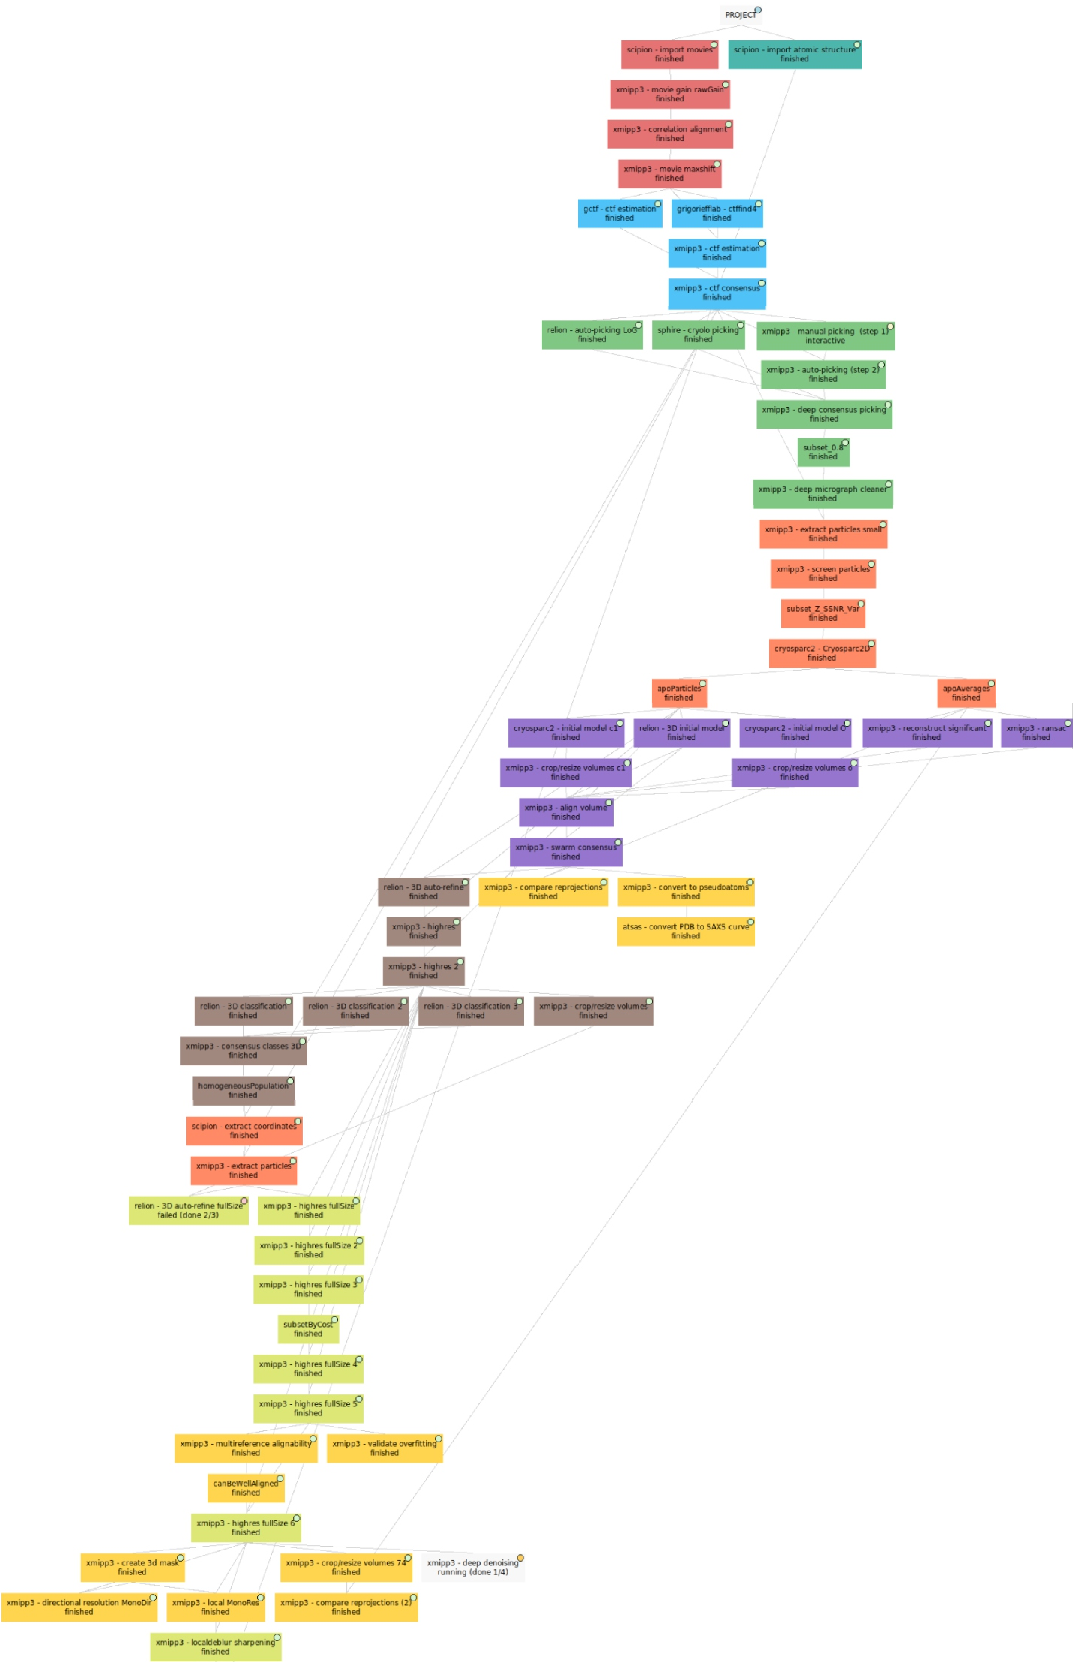
\includegraphics[width=0.95\textwidth]
  {images/workflow.pdf}
  \caption{Apoferritin processing workflow.}
  \label{fig:workflow_pdf}
  \end{figure}






